\section{Background: RP}

\label{background}
\subsection{Rx in a nutshell}
To understand how we create the visualization a minimal understanding of RP and the chosen implementation is required. Many RP implementations share a notion of a \textit{Observable}, which is a collection which abstracts over \textit{time}, in contrast to \textit{space} like standard collections.

Figure \ref{sample1} shows a very basic example of a in situ data flow in Rx. First an \textit{Observable} is created, here using the static \code{from} method, then dependent Observables are created using the \code{map} and \code{filter} methods on the Observable instance. Finally we \code{subscribe} to start the data flow and send the data in the flow to the console (eg. JavaScript's stdout).

\begin{figure}
\inputminted[tabsize=2]{javascript}{listings/sample1.js}	
\caption{Creation and transform of Observables}
\label{sample1}
\end{figure}

It is important to note that the Observable is lazy, it is the blueprint of a data flow. Only when you \code{subscribe} to an Observable the data flow is created by recursively subscribing up the stream. \textit{Observer}s are subscribed to each Observable until the source Observable is reached.
This is illustrated in figure \ref{dualgraphs}.
The origin of this design is the duality between Observables and \textit{Iterables}~\cite{meijer2010subject}, where Observers are dual to \textit{Iterators}.

Creating the Observable we will call the \textit{assembly} phase, the phase where the subscribe happens the \textit{subscription} phase and data flows in the \textit{runtime} phase. The three phases can be interleaved for different streams, for example when dealing with higher order Observables,  meaning one could use Observables as values inside the data flow. The Observables used as values have yet to start the second phase while the outer stream is in the runtime phase.

\begin{figure}
\begin{verbatim}
TODO nice figure with Graph & 2 lines (1 up, 1 down)
^ from(1, 2, 3)   			
^ .map(x => x * 2)       v
^ .filter(x => x > 2)    v
  .subscribe()           v
\end{verbatim}
\caption{Observable \& Observer dependencies}
\label{dualgraphs}
\end{figure}


\begin{figure}[t]
\centering
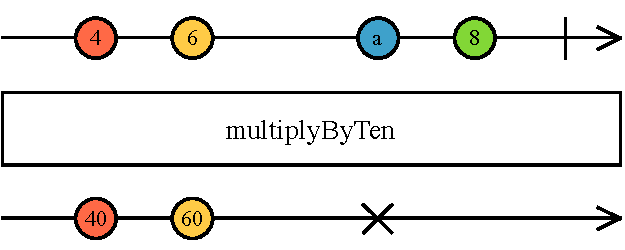
\includegraphics[width=\columnwidth]{images/marble-diagram.pdf}
\caption{Marble Diagram}
\label{marblediagram-image}
\end{figure}

\paragraph{Marble Diagram}
\label{marblediagram}
The term \textit{Marble Diagram} comes from the shape of the glyps in the images used to explain Rx in the official documentation. 
The diagrams contain one or more timelines containing the events that enter and leave Observables. 
Developers can see from the diagram how operators work by inspecting the difference between the timelines, 
where events might be skipped, added, transformed or delayed. 
Mapping time on the x-axis provides insight that is missing when inspecting only a single time slice.
